\usetikzlibrary{arrows.meta,decorations.pathreplacing,patterns}


\ifdefined\codeBoxA\else\newsavebox\codeBoxA\fi
\begin{lrbox}{\codeBoxA}
\lstset{language=C++}
\begin{lstlisting}
void readFromDiskInto(int diskLocation, char *dest) {
    ...
    runPrivilegedInstruction(...);
    ...
}
\end{lstlisting}
\end{lrbox}
\ifdefined\codeBoxB\else\newsavebox\codeBoxB\fi
\begin{lrbox}{\codeBoxB}
\lstset{language=C++}
\begin{lstlisting}
void readFileSafely(const char *name, char *dest) {
    if (canCurrentProgramCanAccessFile(name)) {
        readFromDiskInto(lookupFile(name), dest)
    }
}
\end{lstlisting}
\end{lrbox}

\begin{frame}[fragile,label=callOSDirectP]{calling the OS?}
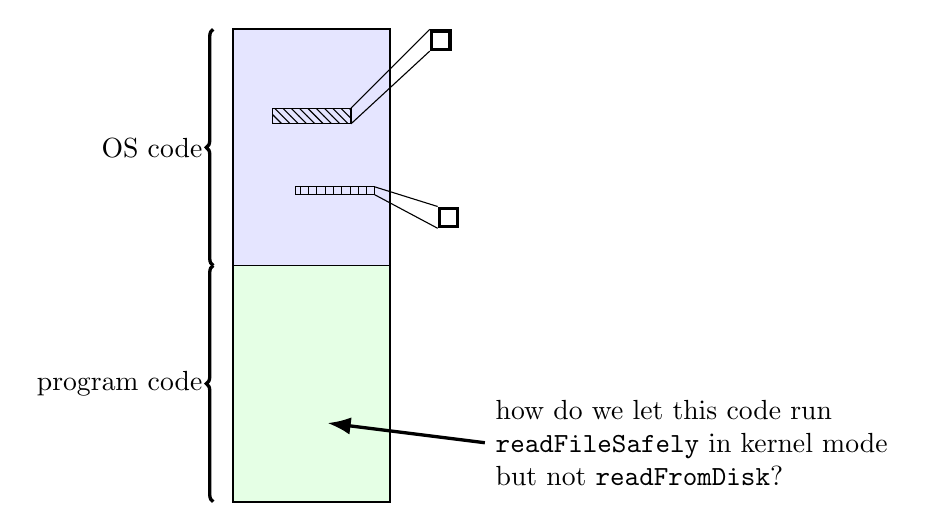
\begin{tikzpicture}
\draw[fill=blue!10] (0, 0) rectangle ++(2, -3);
\draw[fill=green!10] (0, -3) rectangle ++(2, -3);
\draw[thick] (0, 0) rectangle ++(2, -6);
\draw[very thick,decorate,decoration={brace,mirror}] (-.25, 0) -- ++(0, -3)
    node[midway,left] {OS code};
\draw[very thick,decorate,decoration={brace,mirror}] (-.25, -3) -- ++(0, -3)
    node[midway,left] {program code};
% FIXME: pointer to functions in OS
\draw[thin,pattern=north west lines] (0.5, -1) rectangle ++(1.0, -.2);
\draw[thin,pattern=vertical lines] (0.8, -2) rectangle ++(1.0, -.1);
\draw (1.5, -1.0) -- ++(1cm, 1cm) node[draw,very thick,anchor=north west,font=\tt\scriptsize] (readFromDiskInto) {
\usebox{\codeBoxA}
};
\draw (1.5, -1.2) -- (readFromDiskInto.south west);

\draw (1.8, -2.0) -- ++(.8cm, -.25cm) node[draw,very thick,anchor=north west,font=\tt\scriptsize] (readFileSafely) {
\usebox{\codeBoxB}
};
\draw (1.8, -2.1) -- (readFileSafely.south west);

\draw[very thick,Latex-] (1.2, -5) -- ++ (2cm, -.25cm) node[right,align=left] {
    how do we let this code run \\
    \texttt{readFileSafely} in kernel mode \\
    but not \texttt{readFromDisk}?
};
% FIXME: pointer to user code
\end{tikzpicture}
\end{frame}
